\documentclass[a4paper,twoside,openany,notitlepage]{book}
\usepackage[T1]{fontenc}
\usepackage[utf8]{inputenc}
\usepackage[english,italian]{babel}
\usepackage{geometry}
\geometry{a4paper,top=3cm,bottom=3cm,left=2.5cm,right=2.5cm,%
	heightrounded,bindingoffset=5mm}
\usepackage{amsmath}
\usepackage{amssymb}
\usepackage{amsthm}
\usepackage{booktabs}
\usepackage{caption} %per inserire descrizione immagini
%\usepackage{sidecap} %per inserire descrizioni laterali alle immagini
\usepackage{wrapfig} %per inserire immagini a lato pagina, wrappando il testo intorno
\usepackage{graphicx} %impaginazione
\usepackage{blindtext} %boh
\usepackage{isotope} %scrittura isotopi
\usepackage{url} %scrittura di link
\usepackage{hyperref} %collegamenti ipertestuali e link web

%Per l'inserimento immagini la guida molto utile di wikipedia:
%https://en.wikibooks.org/wiki/LaTeX/Floats,_Figures_and_Captions

%Settaggio comandi grafici
%\renewcommand{\caption*}[1]{\begin{center}{\caption*{#1}}}%inserimento testo centrato sotto immagini
\captionsetup{justification=centering}

%Definizione comando email e settaggio del pacchetto hyperref
\newcommand{\mail}[1]{\href{mailto:#1}{\nolinkurl{#1}}}
\hypersetup{hidelinks}

%Definizione comando per notazione vettoriale e simbolo definizione
\renewcommand{\vec}{\boldsymbol}
\newcommand{\Def}{\overset{\mathit{def}}{=}}

%Definizione comando per notazione scientifica
\newcommand{\e}[1]{\cdot 10^{#1}}

%Definizione unità di misura
\newcommand{\angstrom}{\mbox{\normalfont\AA}}

%Funzioni trigonometriche iperboliche ed inverse
\DeclareMathOperator{\sech}{sech}
\DeclareMathOperator{\csch}{csch}
\DeclareMathOperator{\arcsec}{arcsec}
\DeclareMathOperator{\arccot}{arcCot}
\DeclareMathOperator{\arccsc}{arcCsc}
\DeclareMathOperator{\arccosh}{arcCosh}
\DeclareMathOperator{\arcsinh}{arcsinh}
\DeclareMathOperator{\arctanh}{arctanh}
\DeclareMathOperator{\arcsech}{arcsech}
\DeclareMathOperator{\arccsch}{arcCsch}
\DeclareMathOperator{\arccoth}{arcCoth}

%Definizione comandi per teoremi, enunciati ecc
\theoremstyle{definition}
\newtheorem{definizione}{Definizione}
\newtheorem*{definizionenn}{Definizione}
\newtheorem*{principio}{Principio}
\newtheorem*{postulato}{Postulato}
\newtheorem*{exmp}{Esempio}
\newtheorem{exrc}{Esercizio}
\newtheorem{sol}{Soluzione}

\theoremstyle{plain}
\newtheorem{teorema}{Teorema}
\newtheorem*{teoremann}{Teorema}
\newtheorem*{lemma}{Lemma}
\newtheorem*{proprietà}{Si trova che}

\begin{document}
\frontmatter
\author{Volpe Francesco}
\title{Appunti di Astrofisica sperimentale}
%\mail{francesco.volpe1998@gmail.com}
\date{}
\maketitle

\pagestyle{plain}
\tableofcontents

\chapter*{Prefazione}

Il corso di cui si riportano gli appunti è dell'anno accademico 2020/2021 presso l'università di Ferrara ed è suddiviso in tre parti: la prima tenuta dal professore P. Rosati, la seconda tenuta dal professore C. Guidorzi, la terza (prettamente sperimentale) tenuta dal prof E. Virgilli.

I concetti di base del corso sono ripresi e integrati dal corso di Astrofisica del primo semestre del terzo anno, a cui si aggiungono alcuni dettagli sulle misurazioni fotometriche e una trattazione aggiuntiva sulla misurazione delle distanze. Sulle grandi distanze verranno introdotti anche alcuni concetti del corso opzionale di Cosmologia, poiché risulterà impossibile continuare una trattazione classica. Finita la prima parte di trattazione dei telescopi e di tecniche di misura basate sui raggi x e sui "soft" x si passa alla seconda parte del corso, che tratterà la misura di masse, i sistemi binari fino ad arrivare ad accennare alle stelle compatte e i buchi neri, parlerà inoltre di onde gravitazionali, dell'astronomia multi-messaggera (che verrà introdotta nella prima parte del corso) e di tecniche di rivelazione di nuovi pianeti extra-solari. La terza parte tratterà la fisica dei rivelatori e l'astrofisica ad alte energie (quindi oltre i raggi x), la spettroscopia e fondamenti di analisi di X e $\gamma$, con esperienze al LARIX (laboratorio interrato al polo scientifico-tecnologico a Ferrara) e se sarà possibile all'INAF a Bologna.

I libri principalmente usati sarano Astronomy Methods - H. Bradt, Astronomy principles and practice - A.E.Roy \& D. Clarke, Fundamental Astronomy - Kattunen.

\mainmatter

\part{Rosati}

\chapter{Concetti base di osservazioni e misurazioni}

\section{Sonde di informazione}

Spaziamo in varie scale di grandezza, dalle scale scolari fino a quelle intergalattiche.
Le sonde di informazione principali fino a circa il 2015 erano le onde elettromagnetiche, con tutte le loro caratteristiche. Successivamente vennero rivalutati e sempre più utilizzati i raggi cosmici, ossia elettroni, protoni, nuclei pesanti e altre particelle molto energetiche. Una grande aggiunta alle fonti di informazione fu la scoperta dei neutrini cosmici e successivamente quella delle onde gravitazionali, entrambi questi ultimi sono molto difficili da rivelare, ma il loro vantaggio è che subiscono pochissime alterazioni nonostante le gigantesche distanze percorse. Infatti, alcune onde gravitazionali portano informazioni fino al Big Bang, questo le rende, insieme ai neutrini, delle ottime sonde d'informazione, rendendo possibile studiare direttamente la fisica delle fonti, a differenza di quanto avviene con le onde elettromagnetiche, soggette ad un grande numero di perturbazioni e assorbimenti prima di arrivare a noi. Lo spettro di queste ultime viene modificato pesantemente, passando per il mezzo interstellare e il mezzo intergalattico, subisce redshift, scattering, assorbimenti, distorsioni spaziali, cambi della polarizzazione e così via. A questo si aggiungono gli effetti dell'atmosfera nel caso l'osservatorio si trovi sul pianeta e non in orbita, effetti come l'aumento di background dato dalla luminosità del cielo, oltre ad ulteriori distorsioni e assorbimenti. Questo rende chiaramente le onde elettromagnetiche, pur quanto facilmente rivelabili, difficili da trattare, poiché prima di interpretare la fisica della fonte del segnale bisogna fare un ottimo lavoro di comprensione del mezzo che il segnale ha percorso ed elaborare correttamente quest'ultimo. Nel caso di rivelatori a terra, è necessario scegliere la tecnologia di rivelazione e la postazione in cui installare i dispositivi per ridurre al minimo il disturbo atmosferico. L'astronomia multi-frequenza è ora estremamente diffusa e sfruttata per cui è importante ricordarsi i valori della bande in cui si lavora e delle relative energie poiché saranno frequenti i salti dal radio fino ai raggi X.

\begin{figure}[h]
	%figura presa dalle slide
	\centering
	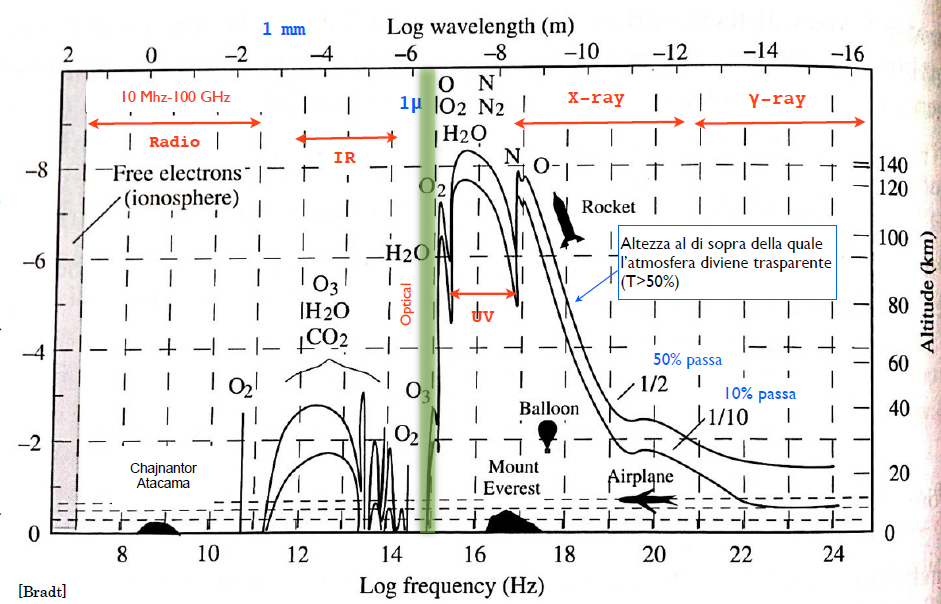
\includegraphics[width=0.8\textwidth]{./Immagini/Capitolo1/trasparenza_atm.png}
	\caption*{Trasparenza atmosferica in funzione della radiazione incidente}
\end{figure}

Vedendo un classico diagramma delle frazioni di atmosfera in funzione delle lunghezze d'onda, avremo due linee, una indica la frazione di atmosfera al di sotto della quale il 50\% della radiazione in quell'ascissa viene schermata, e una seconda linea, più bassa, che indica la porzione di atmosfera necessaria a schermare il 90\%. Si nota che la seconda curva, relativamente ai raggi oltre l'ottico, compresi X e $\gamma$, è fortunatamente ben al di sopra dei $10km$ di quota, cosa che preserva la vita sul pianeta ma al tempo stesso rende necessari satelliti e rivelatori ben al di sopra dell'atmosfera per lo studio di eventi particolarmente energetici e che quindi riguardano principalmente i raggi X e $\gamma$. Per motivi di assorbimento delle molecole presenti nell'atmosfera (azoto molecolare, acqua, ossigeno molecolare, anidride carbonica ecc) si presenta un'assorbimento nullo nella banda del radio ma più interessante ancora la finestra presente nella banda ottica, a cui il nostro occhio si è adattato nel corso dell'evoluzione, finestra che va da $4000\angstrom$ a $9000\angstrom$. Un'altra finestra che ha acquisito interesse negli ultimi anni e in cui l'assorbimento è meno efficiente e a quota minore è quella dell'infrarosso, analizzabile anche tramite palloni aerostatici (pur quanto il satellite rimanga sempre la scelta più fine e con meno disturbo del segnale). Si parla di vicino infrarosso quando si va nel millimetrico, ossia sopra i $500\mu m$, fino ad arrivare alla banda radio che inizia a $2mm$ di lunghezza d'onda. Per questa banda è fondamentale, oltre il raggiungere una buona quota, di trovarsi in un posto molto secco, in quanto il vapore acqueo è estremamente efficiente in questo assorbimento. Il radio non presenta particolari problemi se non a lunghezze d'onda eccessivamente grandi per cui la ionosfera diventa opaca per via dell'assorbimento degli elettroni. Solitamente si parla di energia $h\nu$ dei fotoni o delle frequenze più che delle lunghezze d'onda, soprattutto per le bande maggiori, ma la trattazione rimane analoga e per il radio e infrarosso si continua a parlare anche in termini di lunghezza d'onda $\lambda$. Parlando da un punto di vista storico, la tecnologia astrofisica ha spesso fatto da spin-off per quella bellica, la prima tecnologia ad essersi sviluppata fu quella radio per le comunicazioni durante la seconda mondiale, così come per gli X relativamente all'osservazione di eventuali esplosioni di ordigni atomici negli anni '50 e '60, negli anni '90 si sviluppò quella infrarossa e i detector a stato solido, questi ultimi furono di impatto fondamentale sulla qualità delle analisi nell'ottico e nell'infrarosso. I primi rivelatori a stato solido (SSD - solid state detector) coprivano 256 pixel, mentre oggi ci sono camere intere che coprono dei gigapixel. Per le singole bande esistono poi grafici più specifici descriventi l'assorbimento relativo in funzione della lunghezza d'onda a quota fissata.

\begin{wrapfigure}{r}{0.5\textwidth}
	%figura presa dalle slide
	\vspace{-8pt} %toglie lo spazio bianco in eccesso che figure e centering mettono
	\centering
	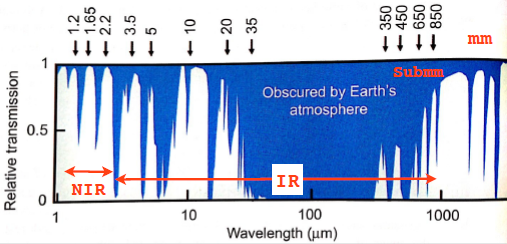
\includegraphics[width=0.4\textwidth]{./Immagini/Capitolo1/trasparenza_atm_IR.png}
	\vspace{-5pt}
	\caption*{Trasparenza atmosferica nell'infrarosso e vicino infrarosso}
	\vspace{-8pt}
\end{wrapfigure}

Si nota nel grafico come ci siano varie finestre nel vicino infrarosso, corrispondenti alle parti di banda non oscurate, e che combaciano di fatti con i filtri J, H, K appositamente tarati, cosa peculiare degli IR, mentre nell'ottico non avendo assorbimento possono essere costruiti filtri secondo criteri di comodità. Le osservazioni si fanno particolarmente difficili da terra per onde oltre i $2\mu m$, poiché la luminosità del cielo va a creare un background troppo fastidioso per fotoni così poco energetici, per cui si arriva ad avere troppo contrasto nelle rivelazioni. Per questo, i siti astronomici devono essere messi lontani dalle città, per via del loro grande inquinamento luminoso, oltre che ad alta quota e in luoghi secchi, per altri motivi che discuteremo i siti migliori sono sulle isole o nelle coste occidentali dei continenti per via della costanza degli eventi ad alta quota (i venti tirano da ovest a est e così facendo sopra gli osservatori non passano eventi che hanno attraversato la terra), o ai poli per via della quota e dell'aria molto secca.

Un fattore molto importante è quello della luminosità del cielo, soprattutto per le fonti più deboli, che esse siano puntiformi o meno, e si introduce il concetto di brillanza superficiale del cielo per quantificare questo fattore di disturbo. Concetto base per introdurre la brillanza è quella di magnitudine, che è il flusso elettromagnetico per unità di angolo solido osservato. Per quantificare il fondo del cielo, si può prendere un secondo d'arco di cielo, o equivalentemente un grado sessagesimale e dividerlo poi per 3600, e poi misurare il flusso in sola quella porzione di cielo, facendo il rapporto esce quanto cercato. Ci si chiede come mai di notte non si osservi un cielo completamente nero e questo è dovuto in parte, nelle zone più isolate, prevalentemente a fonti di origine extra-terrestre, di cui la principale è la luce zodiacale. Dalla formazione del sistema solare e dei pianeti è rimasta una nube di gas e detriti proto-solare (silicati e materiali pesanti, di dimensione molto varia) che si trova sullo stesso piano dei pianeti e del Sole (l'eclittica) per conservazione del momento angolare (essendo che si è formato prima il sole e successivamente dai detriti i pianeti).

\begin{figure}[h]
	%figura presa dalle slide
	\centering
	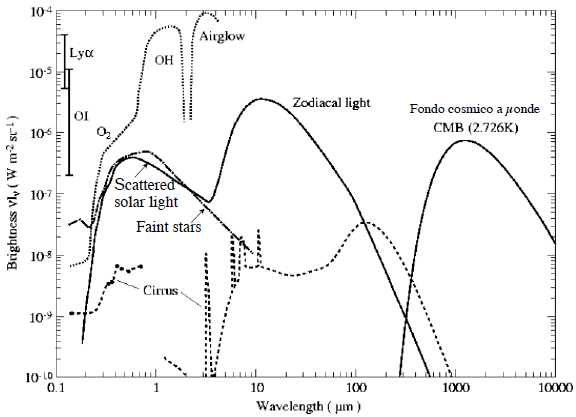
\includegraphics[width=0.6\textwidth]{./Immagini/Capitolo1/brillanza_sup_cielo.png}
	\caption*{Fonti della brillanza superficiale del cielo}
\end{figure}

Questa polvere si trova tra i $250K$ e i $300K$ e viene illuminata dai raggi solari, nella banda dell'ottico, da qui la cosiddetta luce zodiacale, con picco del flusso sui $3\mu m$ per via della propria emissione in quanto corpo nero, e con picco tipico del flusso solare (a circa $0.9\mu m$) per quanto riguarda lo scattering dei raggi provenienti dal sole, il quale è anch'esso un corpo nero. Di fatti la curva in entrambi i punti segue quella del corpo nero essendo la sovrapposizione di due flussi emittenti di corpi neri, perciò risulta particolarmente importante per il trattamento dell'irraggiamento termico conoscere la legge di Wien. Oltre a questo fattore c'è anche il fondo cosmico, il più perfetto corpo nero misurato, dato dal Big Bang e dominante sul fondo nella banda del millimetrico, inoltre c'è il mezzo intergalattico illuminato da stelle particolarmente luminose, più fredde del sole, che danno un contributo minore in ordini di grandezza ma comunque rilevante al fondo. Mettendosi nel sistema di riferimento dell'eclittica (che si ricorda essere la traiettoria del Sole vista dalla Terra), ossia prendendo asse x e y sull'eclittica e asse z perpendicolare a tale piano, prendendo come origine l'equinozio vernale, si possono fare osservazioni meno disturbate dalla luce zodiacale andando verso il polo nord eclittico, che sarà il punto più lontano dall'eclittica e quindi dalla serie di detriti che generano il rumore di fondo.

Un secondo contributo alla brillanza superficiale del cielo è dato dai fattori di origine terrestre: air glow, aurora boreale (frutto dell'attività solare), emissione termica del pianeta, luce lunare diffusa, inquinamento luminoso dato dalle attività umane (di grande disturbo, per questo i siti di osservazione sono molto isolati), nano-satelliti in orbita (ad esempio di Google, Space X ecc, che vanno a mettersi in mezzo alla linea di osservazione durante le misurazioni e sono in aumento giornaliero vertiginoso). Il primo fattore riguarda le molecole e gli atomi presenti in atmosfera, soprattutto negli strati più alti, e si tratta dell'emissione a righe (secondo i vari spettri atomici) a seguito dell'irraggiamento che subiscono dai fotoni in arrivo dallo spazio, questa componente è particolarmente di disturbo da terra e possiede sia una componente spettrale a righe che una parte continua di fondo. L'emissione termica è la semplice emissione del pianeta in quanto corpo nero, il cui picco di emissione, data la temperatura, si attesta su qualche micron, i prossimi satelliti verranno per questo inviati a milioni di km dalla Terra, poiché fonte di grande rumore di fondo per le osservazioni oltre il vicino infrarosso, come è stato osservato dalle acquisizioni del telescopio spaziale Hubble.

\section{Misure fotometriche}

\subsubsection*{Sorgenti puntiformi}
Prendiamo una sorgente puntiforme con emissione elettromagnetica isotropa, si definisce \textbf{densità spettrale di flusso} l'energia raccolta per unità di superficie collettrice, di tempo e di banda di frequenza passante, essendo che sarà un'emissione a spettro si deve distinguere per le varie bande analizzate:
\begin{equation*}
	dE=S_\nu dAdtd\nu
\end{equation*}
Le unità di misura cambiano a seconda della banda per comodità, solitamente per il radio si usa il Jansky ($1 Jansky = \e{-26} W/m^2/Hz$). Per i raggi X e $\gamma$ si usa l'energia invece che l'unità di banda e si adopera $erg/cm^2/s$, passando quindi alla \textbf{densità di flusso}, definita come la densità di flusso spettrale integrata sulla specifica banda di frequenze:
\begin{equation*}
	\Phi=F_{\Delta\nu}=\int_{\Delta\nu}^{}S(\nu)d\nu = S_{mean}\Delta\nu
\end{equation*}
Si definisce da qui la densità di flusso di fotoni come il rapporto tra la densità di flusso in una banda e l'energia media specifica di quella banda:
\begin{equation*}
	\Phi_{ph}=\frac{F_{\Delta\nu}}{<E>}
\end{equation*}
Bisogna fare attenzione al cambio tra unità di frequenza e unità di lunghezza d'onda:
\begin{equation*}
	S_\nu d\nu = S_\lambda d\lambda, \quad \lambda=\frac{c}{\nu} \quad \longrightarrow \quad
	S_\nu = -S_\lambda \frac{\lambda^2}{c}, \quad S_\lambda = -S_\nu \frac{\nu^2}{c}
\end{equation*}
Si continua introducendo la \textbf{potenza ricevuta} da un'antenna ricevente come l'integrale della densità di flusso spettrale sull'area collettrice nella specifica banda:
\begin{equation*}
	P=A_{eff}\int_{\Delta \nu}^{} S(\nu)d\nu
\end{equation*}
Espressa in $W$, si tiene conto delle efficienze delle componenti costituenti i detector nel termine $A_{eff}$ con cui si intende l'area efficace alla rivelazione.
Si passa alle misure fotometriche in relazione alle sorgenti stesse col definire il concetto di \textbf{luminosità}: questa è l'energia emessa per unità di tempo e in una determinata banda, che per una sorgente isotropa diventa
\begin{equation*}
	L_{\Delta\nu} =F_{\Delta\nu} \cdot 4\pi R^2, \quad R=\text{distanza sorgente}
\end{equation*}
Dove il termine di superficie deriva dalla superficie sottesa dall'angolo solido che ha come vertice la sorgente puntiforme, tiene in questo modo conto della "diluizione" dell'energia nello spazio in cui viene irradiata. Questo concetto si estende alla cosiddetta \textbf{luminosità bolometrica} nel momento in cui si trattano tutte le bande di emissione di una stessa sorgente:
\begin{equation*}
	L_{bol} = 4\pi R^2 \int_{-\infty}^{+\infty} F(\nu) d\nu
\end{equation*}
Una costante importante nel nostro sistema è la \textit{costante solare}, che è la potenza emessa per metro quadro subito al di sopra della nostra atmosfera, che è pari a $1366W/m^2$, da qui per trovare la luminosità del Sole rispetto al nostro pianeta è sufficiente moltiplicare per $4\pi R^2$, dove $R$ diventa la distanza tra la terra ed il Sole, $R=1.5\e{11}m$ (altra costante abbastanza ricorrente), da cui la luminosità bolometrica del Sole è $L_\odot=3.8\e{26}W$. Prendendo un esempio, se si considera una sorgente radio al centro galattico, con densità di flusso tipica di queste sorgenti $F_{50-150MHz}=1Jy$, avrà una luminosità data dalla definizione di luminosità per sorgenti isotrope, dove si ricorda che $1Jy=1\e{-26}W/m^2$, che la distanza tra la Terra e il centro galattico è $R=2.4\e{20}m$ e che $\Delta\nu=1\e{8}Hz$, da cui $L_{radio} = 1\e{-26} \cdot 1\e{8} \cdot 4\pi \cdot (2.4\e{20})^2=7\e{23}W$. Lo stesso discorso può essere fatto per il quasar 3C273 alimentato da un buco nero a distanze cosmologiche ($R=749Mpc=749 \cdot 3\e{22}m$), dove $F_\nu=100Jy$ nella banda $0.1-1GHz$, da cui la sua luminosità nel radio è $L_{radio} = 100\e{-26} \cdot 900\e{6} \cdot 4\pi (749 \cdot 3\e{22})^2 = 5\e{36}W$, mentre $L_{bol} = 10^{38}W\sim10^{12}L_\odot$.

Concentrandoci sullo spettro solare, ci saranno due curve, una misurata in orbita e che approssimerà meglio l'andamento di un corpo nero ideale, mentre una misurata da terra, la quale è notevolmente diversa, sia più schiacciata per via della schermatura data dai vari strati dell'atmosfera sia frastagliata di righe di assorbimento corrispondenti alle righe di assorbimento delle molecole presenti in atmosfera. Integrando la curva dello spettro di irradiazione al di fuori dell'atmosfera si ottiene la citata costante solare pari a $1366W/m^2$, mentre integrando quella ricevuta a terra si trova circa $1kW/m^2$. Chiaramente questo valore non è sempre costante così come non lo è il sole, la cui superficie è contraddistinta dalle sue macchie solari che sono zone di depressione magnetica in cui il gas è più freddo, dando valori di potenza in emissione oscillanti nel tempo, sia su scale annue che giornaliere, e il cui valore medio è la costante trovata.

\subsubsection*{Sorgenti estese}
Passando alle sorgenti estese, il concetto di flusso spettrale va esteso ad un elemento della superficie emittente, introducendo il concetto di \textbf{intensità specifica} $I_\nu (\theta,\phi)$, definita come la densità di flusso ricevuta per unità di angolo solido $d\Omega$ nella direzione $\theta,\phi$ (l'angolo può essere espresso in steradianti come in arcosecondi), dove nell'integrazione dell'area bisogna considerare l'area normale alla direzione di emissione ed è stato introdotto un sistema di riferimento solidale all'osservatore.
\begin{equation*}
	S(\nu)=\int_{\theta}^{}\int_{\phi}^{} I(\theta,\phi,\nu)\cos\theta d\Omega
\end{equation*}
Questa specificità deriva anche dal fatto che un corpo esteso ammette la possibilità di emettere in maniera non isotropa. Da questa definizione deriva quella di \textbf{brillanza superficiale osservata} $B_{obs}$, ossia la densità di flusso misurata in una certa banda per unità di angolo solido di osservazione:
\begin{equation*}
	B_{obs} = \frac{F}{\Delta\Omega} = \frac{L}{4\pi R^2}\frac{R^2}{\Delta S} =
	\frac{L}{4\pi\Delta S}
\end{equation*}
La cui caratteristica più interessante sia come questa quantità non dipende dalla distanza a cui si trova il corpo rispetto l'osservatore. Un'altra unità basata invece sulle caratteristiche della fonte più che sulla sua osservazione è la \textbf{brillanza superficiale emessa} $B_{em,\nu}(\theta,\phi)$, definita come la potenza irradiata per unità di superficie emittente e unità di frequenza e di angolo solido $d\Omega$ nella direzione $(\theta,\phi)$. Un esempio tipico di quest'ultima quantità e di come la si possa usare per calcolare il flusso emesso è considerare la superficie di una stella, in cui ogni sezione della sua superficie emetterà come un corpo nero, da cui il flusso emesso sarà dato da:
\begin{equation*}
	F_\nu = \int_{\Omega}^{} B_{em,\nu} \cos\theta d\Omega =
	\int_{0}^{2\pi} \int_{0}^{\frac{\pi}{2}} B_{em,\nu} \cos\theta\sin\theta d\theta d\phi =
	\pi B_{em,\nu}
\end{equation*}
Dove per gli estremi di integrazione si considera necessariamente un solo emisfero alla volta, in quanto una stella irradia chiaramente solo in uscita, e in cui è considerata la sezione di superficie ortogonale la direzione di emissione. Trattandosi di un corpo nero, la sua brillanza superficiale emessa avrà la seguente forma:
\begin{equation*}
	B_{em,\nu} (T) = \frac{2h\nu^3}{c}\frac{1}{e^{h\nu/kT}-1}
\end{equation*}
La densità di flusso $F_\nu$ trovata è però in unità di frequenza, integrando su tutte le frequenze troviamo quella che è la luminosità per unità di area emittente:
\begin{equation*}
	\frac{dL}{dA} = \int_{0}^{\infty} F_\nu d\nu =
	\frac{2\pi}{c^2}h \biggl( \frac{kT}{h} \biggr)^4 \int_{0}^{\infty} \frac{x^3 dx}{e^x-1} =
	\sigma T^4 \qquad \text{dove} \quad
	\sigma = \frac{2\pi^5k^4}{15c^2h^3} = 5.67\e{-8}W/m^2/K^4
\end{equation*}
Che altri non è che la \textbf{legge di Stefan-Boltzmann}, dove $\sigma$ è la costante di nome analogo (per lo svolgimento si ricorda che l'integrale in $dx$ da $\pi^4/15$). Ne consegue che per un oggetto sferico come una stella, considerando $R$ il suo raggio, la potenza totale emessa sarà data da:
\begin{equation}
	\label{eq:Stef-Boltz}
	L = 4\pi R^2 \sigma T^4
\end{equation}

\subsubsection*{Magnitudine e colore}
Dal flusso si introduce una scala storica di utilizzo molto diffuso in astronomia e risalente nella sua prima definizione a Ipparco, introdotta in modo da risultare più comoda e lineare rispetto alla sensibilità dell'occhio umano, che risponde in maniera logaritmica alla sollecitazione luminosa, dovendosi adattare ad un vastissimo range di luminosità, passando dal buio della notte fonda alle giornate più soleggiate. Da Ipparco è stato poi esteso da Pogson nella seconda metà del diciannovesimo secolo ed è una scala inversa, in cui una magnitudine minore significa un flusso, e quindi una luminosità, maggiore (in una certa banda), in cui una differenza di 5 magnitudini corrisponde a una differenza di flusso di un fattore 100, ossia due ordini di grandezza maggiore o minore:
\begin{equation*}
	m_1-m_2 = -2.5log_{10}\frac{F_1}{F_2} \quad \longrightarrow \quad \frac{F_1}{F_2} = 10^{0.4(m_2-m_1)}
\end{equation*}
Dove i flussi $F$ sono quelli rivelati in una certa banda (isolata tramite filtro), pesati per la funzione di risposta $\psi(\nu)$ del mezzo di rivelazione e del telescopio (inclusa l'estinzione atmosferica). Questi filtri classicamente dividono in tre gruppi le bande di studio di maggiore interesse e sono le UBV, U sta per ultravioletto, B per il blu e V per il visibile.
In tempi moderni, è stato necessario definire una magnitudine zero di riferimento, da sostituire al posto di $m_2$ in modo da avere un riferimento standard, e questo compito è stato assegnato alla stella Vega, per cui la magnitudine di un oggetto diventa:
\begin{equation*}
	m = -2.5\log\frac{F}{F_{Vega}} + 0 \qquad \text{dove} \quad
	m_{Vega} = -2.5 \biggl[ \log\int R(\lambda)f(\lambda)d\lambda - \log\int R(\lambda)f_{Vega}(\lambda)d\lambda \biggr]
\end{equation*}
Che è l'integrale dello spettro della stella Vega, particolarmente calda, che nel sistema UBV ha magnitudine $m=0.03$ in tutte e tre le bande. Con diversi telescopi, di grandi dimensioni con raggi di $8m$, riusciamo ad arrivare ad osservare oggetti a magnitudini molto alte, ad esempio riusciamo a rivelare con un'ora di esposizione oggetti a magnitudine 25, aumentando l'esposizione a dieci ore anche oggetti a magnitudine 27, fino a telescopi spaziali che con un paio di settimane di integrazione arrivano a magnitudine 30. Per passare da magnitudini a flussi per ogni banda tra le varie unità di misura ci sono tabelle apposite molto comode. Vedendo le tabelle delle varie magnitudini in banda da osservatori a terra ed osservatori in orbita, si nota come la luminosità del cielo sia minore per un osservatore in orbita, per via dell'effetto dell'atmosfera, particolarmente efficace nella schermatura nel vicino infrarosso, motivo per cui, come anticipato, in orbita è molto conveniente e vengono rivelazioni molto più pulite nella banda del vicino infrarosso, a differenza della situazione a terra che è totalmente opposta per questa stessa banda. Nello spazio la brillanza superficiale del cielo è perciò data essenzialmente dalla luce zodiacale.

\begin{wrapfigure}{r}{0.4\textwidth}
	%figura presa dalle slide
	\vspace{-15pt}
	\centering
	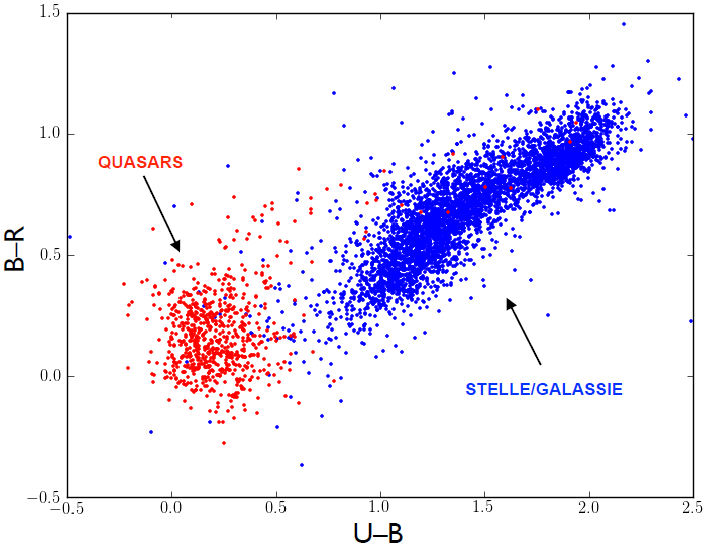
\includegraphics[width=0.39\textwidth]{./Immagini/Capitolo1/diag_col-col_quasar_stelle.PNG}
	\vspace{-5pt}
	\caption*{Diagramma colore-colore di Quasar e stelle}
	\vspace{-15pt}
\end{wrapfigure}

Si introduce il concetto di colore, definito come la differenza di magnitudine di un corpo in due filtri, o bande, successive, questo da appunto un'indicazione del colore della stella tratta, nel caso la differenza tra il filtro U e B sia positiva, vorrà dire che la magnitudine in B sarà minore e la stella avrà quindi un colore tendente più al blu. Un'applicazione interessante di questo parametro è il suo utilizzo nella classificazione delle galassie e sorgenti cosmiche, come i quasar, particolarmente blu per la loro emissione tipica (non di natura termica come può essere quella del Sole), mentre stelle e galassie si collocano più sul rosso. Questo dato, molto utile per capire la temperatura di una stella, può essere anche usato in relazione alla luminosità delle sorgenti stesse, dando il famoso e molto utilizzato diagramma HR (Hertzsprung-Russell):

\begin{figure}[h]
	%figura presa da Wikipedia
	\centering
	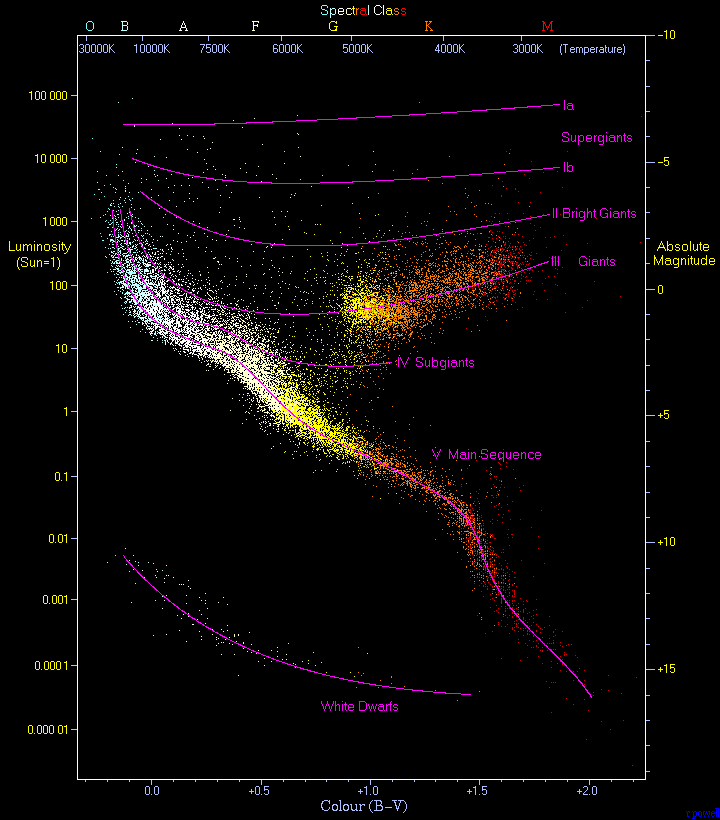
\includegraphics[width=0.6\textwidth]{./Immagini/Capitolo1/Diagramma_HR.png}
	\caption*{Diagramma Hertzsprung-Russell}
\end{figure}

Dove il colore B-V è posto in ascissa e la luminosità in ordinata, in cui si vede un andamento ben preciso lungo una diagonale della maggior parte delle stelle presenti nel grafico, andamento dovuto alla fusione dell'Idrogeno in Elio nelle stelle e descritta dalle equazioni della struttura stellare, che tracciano questa curva come evoluzione temporale di ogni stella.

Trattando le sorgenti astrofisiche, quando si parla di estinzione si deve distinguere tra l'estinzione "spaziale" che avviene nei mezzi intergalattico e interstellare prima che i fotoni arrivino, e quella che invece è dovuta all'atmosfera e di grande impatto nei siti di rivelazione posti a terra. Il fenomeno dell'estinzione atmosferica è una cosa di cui abbiamo esperienza tutti i giorni quando la luce solare deve attraversare grandi strati dell'atmosfera, come succede ad esempio al tramonto, mentre allo Zenit il fenomeno è minimizzato.

\begin{wrapfigure}{l}{0.5\textwidth}
	%Immagine presa da slide
	\vspace{-10pt}
	\centering
	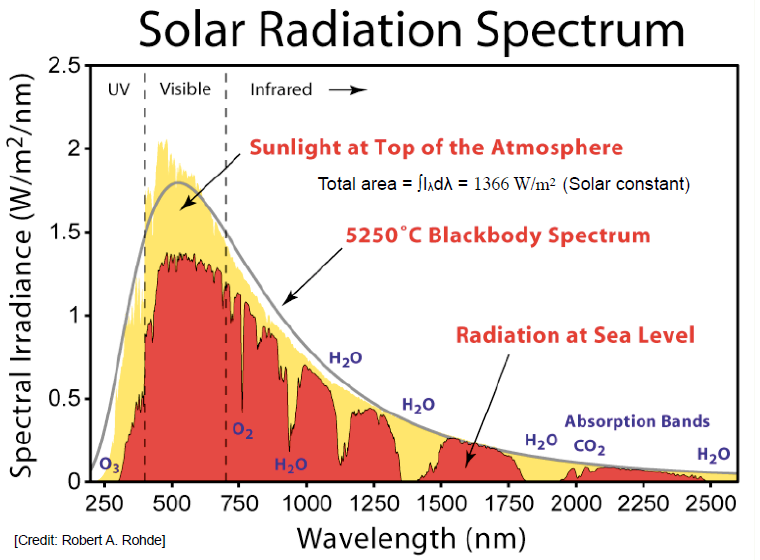
\includegraphics[width=0.49\textwidth]{./Immagini/Capitolo1/Estinzione_atm_sole.png}
	\vspace{-10pt}
	\caption*{Estinzione atmosferica solare}
\end{wrapfigure}

Il fenomeno prende questo nome dal fenomeno stesso, ossia dall'estinzione vera e propria del flusso incidente, dovuto al ripetuto assorbimento e scattering dei fotoni spaziali incidenti sulle molecole atmosferiche, che sarà quantificabile in modo proporzionale alla distanza zenitale e conseguentemente alla porzione di atmosfera che il fascio deve attraversare, data $m_0$ la magnitudine di una stella fuori l'atmosfera:
\begin{equation*}
	m(\zeta) = m_0 + \Delta m \sec \zeta
\end{equation*}
Dove $\sec\zeta$ è detta \textit{massa d'aria} ed è la costante di proporzionalità dell'estinzione, e rappresenta quanta massa d'aria aggiuntiva debba attraversare il fascio rispetto a $dz$ (vedere grafico per capire), dove $\zeta$ è l'angolo che esprime la distanza zenitale. Essendo che lo scattering a cui si assiste è di tipo elastico si sta trattando uno scattering di Rayleigh, il cui fascio diffuso ha intensità $I \propto I_0 \lambda^{-4}$ rispetto all'intensità $I_0$ del fascio incidente con lunghezza d'onda $\lambda$, ciò significa che questo tipo di scattering interessa di più le bande a frequenza maggiore come il blu, di fatti il sole al tramonto tende di più al rosso. Di questa cosa si tiene conto tramite il parametro introdotto in formula che ha valori $\Delta m = 0.6, 0.3, 0.2$ rispettivamente per U, B e V; per cui l'andamento lineare dell'estinzione da pendenze diverse per bande diverse, infatti andando nel vicino infrarosso l'estinzione è quasi trascurabile a meno che non faccia una rivelazione a distanze zenitali particolarmente grandi.

Fin'ora si è trattata la magnitudine "apparente" dei corpi celesti, essendo che queste non tenevano conto della distanza a cui l'oggetto rivelato si trovi, definendo la magnitudine come rapporto dei flussi ricevuti. Chiaramente aumentando la distanza, per i fattori trattati, il flusso ricevuto sarebbe minore e conseguentemente la magnitudine di quel corpo aumenterebbe, per questo motivo si introduce il concetto di \textbf{magnitudine assoluta} $M$, volta ad essere una misura direttamente proporzionale la luminosità e definita come la magnitudine che avrebbe la stella tratta se fosse posta ad una distanza standard di $10pc$ (parsec) rispetto l'osservatore:
\begin{equation}
	\label{def:mag-abs}
	\mu \Def m-M = -2.5 \log_{10} \frac{F}{F_{10pc}} =
	-2.5 \log_{10} \frac{10}{d_{pc}} =
	5\log d_{pc}-5 \quad \longrightarrow \quad
	d = 10^{0.2(m-M)} \cdot 10pc
\end{equation}
Questo appena introdotto è detto \textit{modulo di distanza} e si è definito nell'ipotesi di assorbimento nullo, di fatti è un parametro che dipende dal filtro utilizzato e dovrebbe includere l'effetto dell'assorbimento interstellare per essere considerabile una misura della distanza vera a cui si trova la stella, nel caso del sole $M_{\odot,V}=4.82$. Invertendo la formula, si ha uno strumento molto utile di classificazione delle stelle osservate e di calcolo della distanza a cui esse si trovino, isolando ad esempio una stella nella galassia di Andromeda con lo Space Telescope, nota la distanza esprimibile tramite il modulo di distanza e misurata la magnitudine apparente si trova la magnitudine assoluta $M=m-\mu=4.6$, molto simile a quella solare! Lo stesso è possibile fare con le galassie, prendendone una simile alla nostra, composta da $10^{11}$ stelle e partendo dalla sua luminosità $L_B=10^{10}L_\odot$:
\begin{equation*}
	M_B = -2.5 \log \biggl( \frac{10^{10}L_\odot}{L_\odot} \biggr) + M_{\odot,R} = -25 +5.5 =-19.5
\end{equation*}
Si conclude deducendo il concetto di \textbf{magnitudine bolometrica} come estensione a tutto lo spettro del concetto di magnitudine assoluta:
\begin{equation*}
	M_{bol}=M_V+BC
\end{equation*}
Dove il termine additivo $BC$ è la cosiddetta \textit{correzione bolometrica}, sapendo che $M_{\odot,bol}=4.74$, si deduce che
\begin{equation*}
	M_{bol} = -2.5 \log \biggl( \frac{L}{L_\odot} \biggr) + 4.74 \qquad
	\text{con} \quad L_\odot=3.845\e{26}W
\end{equation*}

\section{Misure e scale delle distanze}

Fintanto che si tratta il sistema solare, di dimensioni decisamente ridotte rispetto all'universo nella sua interessa, si definisce \textit{l'unità astronomica} come la distanza media tra la Terra e il Sole: $1AU=1.5\e{11}m$. Un'altra unità di distanza introdotta, di dimensioni decisamente maggiori rispetto l'unità astronomica, è il \textit{parsec}: $1pc=206265AU=3\e{16}=3.6ly$. Definendo il sistema solare come la zona dello spazio fino a cui il Sole, con i propri venti, riesce ad avere un'influenza dinamica sui corpi al suo interno, allora si trova l'eliosfera, non perfettamente sferica e di raggio pari a circa $100AU$, distanza a cui si sono spinti i telescopi lanciati negli anni settanta Voyager 1 e 2, i quali dovranno arrivare a un milione di unità astronomiche prima di incontrare la prossima stella.

Si ridefinisce il parsec e si introduce il concetto di \textbf{parallasse trigonometrica}, metodo matematico di indagine che svelò per primo le scale della nostra galassia, introdotto da E. Bessel nella prima metà del diciannovesimo secolo. Prima di questo metodo si supponeva che le stelle fossero luminose tanto quanto il Sole, per cui sarebbe bastato misurarne il flusso e tramite la magnitudine assoluta ricavare la distanza, metodo chiaramente errato in quanto le stelle nell'universo possono essere anche estremamente più luminose della nostra.

\begin{wrapfigure}{l}{0.5\textwidth}
	%figura presa dal bradt - astronomy methods
	\vspace{-10pt}
	\centering
	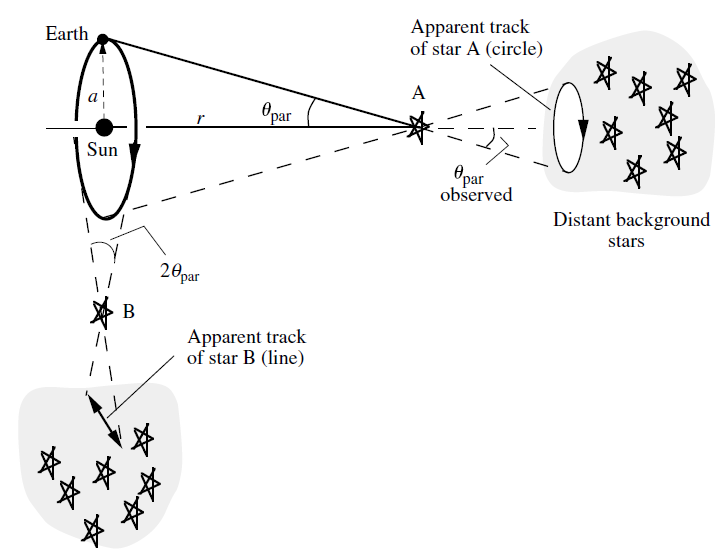
\includegraphics[width=0.49\textwidth]{./Immagini/Capitolo1/parallasse.png}
	\caption*{Visualizzazione della tecnica di parallasse}
	\vspace{-10pt}
\end{wrapfigure}

Questo metodo geometrico, particolarmente utile per le stelle più vicine al nostro sistema, si basa sul moto circolare apparente che esse compiono rispetto ad un osservatore a terra per via del moto di rivoluzione terrestre, infatti ruotando la Terra attorno al Sole, la stella sembrerà compiere nel cielo una rotazione sul piano ortogonale e centrato nella congiungente tra lei e il Sole. Essendo il periodo di rivoluzione del nostro pianeta annuo, prendere misure della posizione della stella a distanza di sei mesi l'una dall'altra permette di calcolare la distanza a cui essa si trova secondo la seguente:
\begin{equation}
	\label{def:parallasse}
	\tan\theta_{par} \simeq \theta_{par} = \frac{a}{r}
\end{equation}
Da cui deriva la definizione formale di parsec, come la distanza alla quale la stella ha parallasse di un arcosecondo
\begin{equation*}
	1\,pc \Def 1\,UA \cdot 206265 = 3.26\,ly \qquad \text{dove} \quad
	1\,arcsec = \frac{\pi}{180} \cdot 3600^{-1} = 206265^{-1} rad
\end{equation*}
Dove la seconda rappresenta il rapporto di conversione da arcosecondi ($1\,arcsec=3600^{-1 \circ}$) a radianti, unità in cui vengono espressi gli angoli all'interno della tangente, ne deriva che:
\begin{equation*}
	D(pc) = \frac{1}{\theta(arcsec)}
\end{equation*}
Le applicazioni di questa tecnica hanno dato la possibilità di fare osservazioni a distanze inimagginabili all'epoca, oggi abbiamo macchine che arrivano ad avere una risoluzione del decimo di milliparsec che permettono di fare sondaggi (surveys) estremamente precisi su ampia scala.

\begin{wrapfigure}{l}{0.5\textwidth}
	\vspace{-5pt}
	\centering
	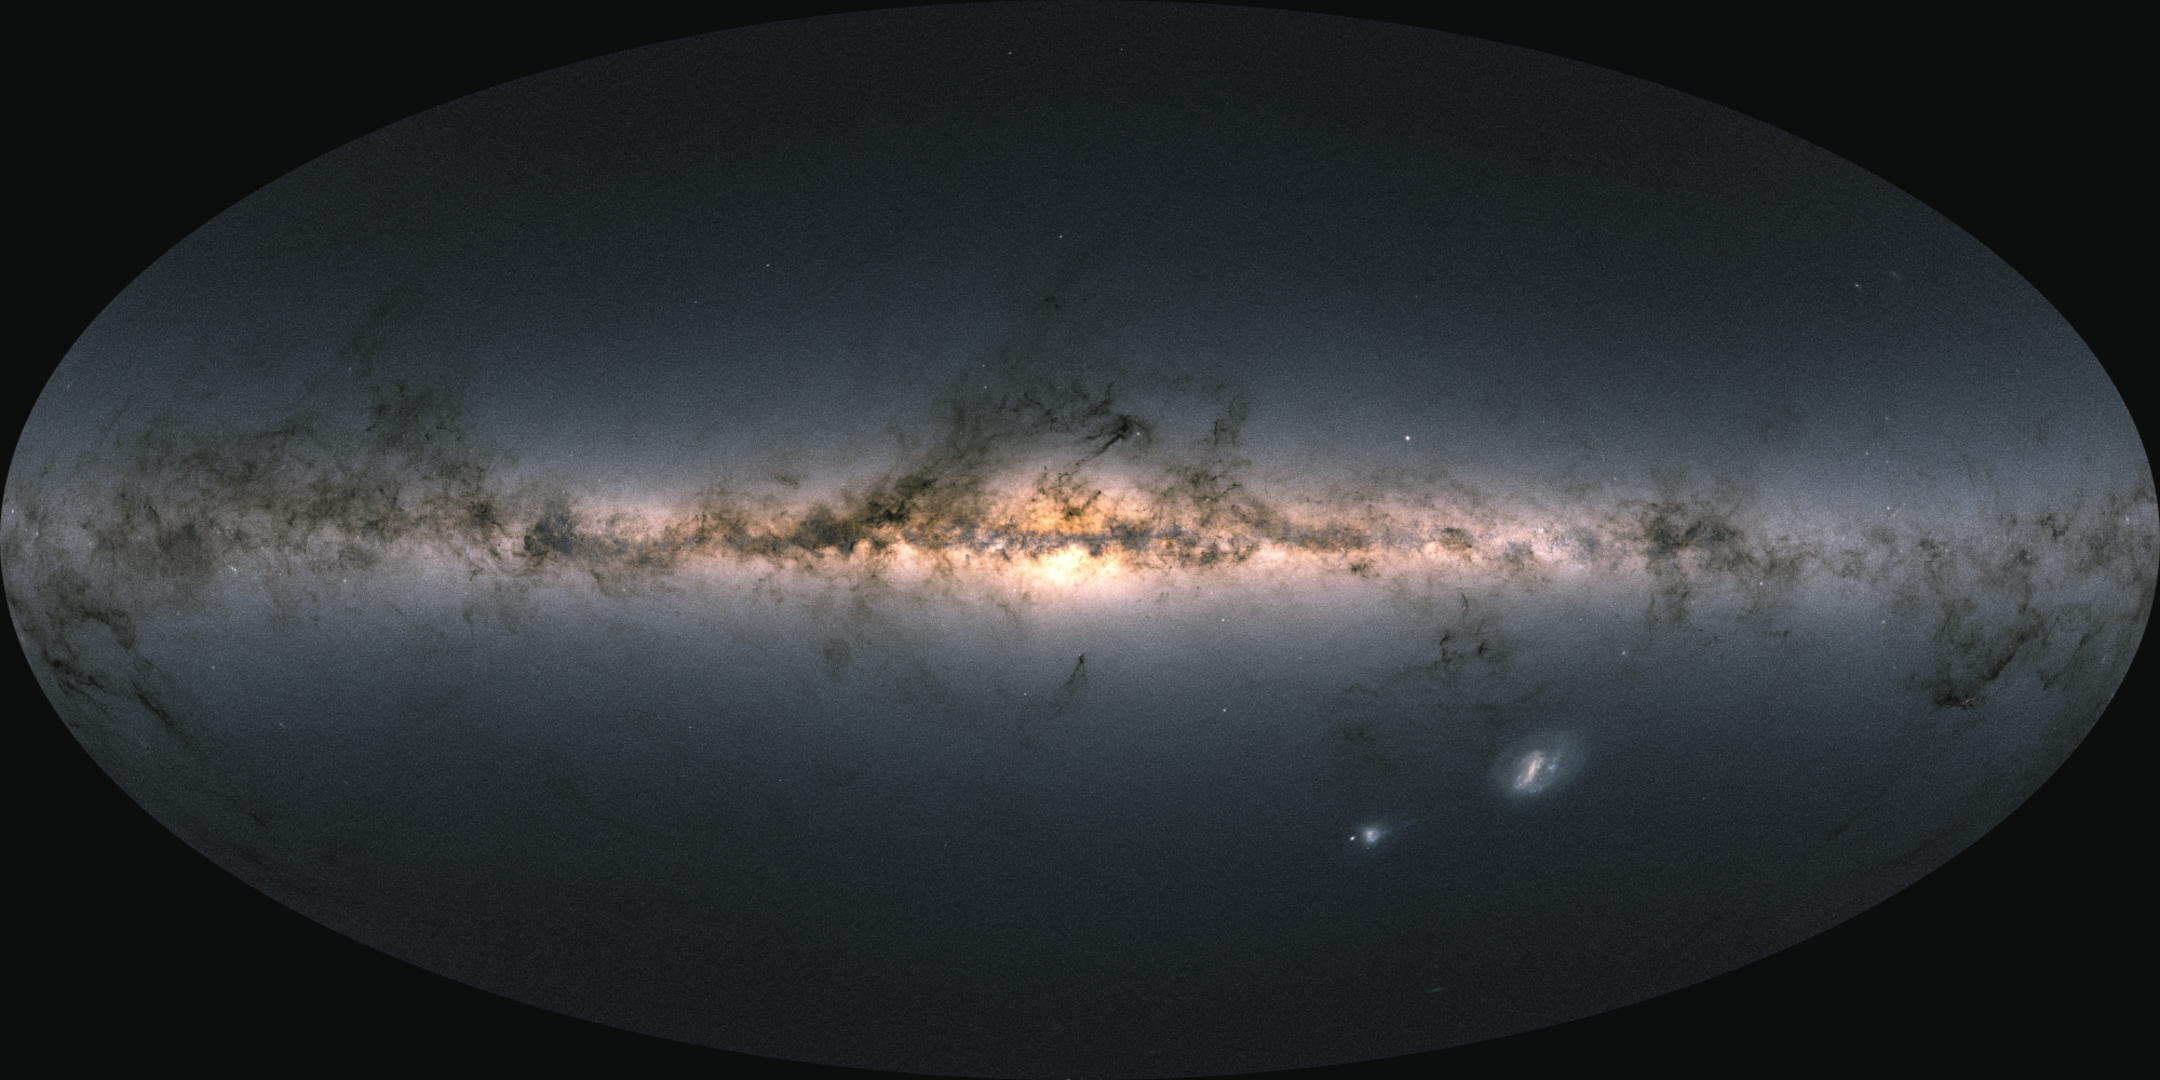
\includegraphics[width=0.49\textwidth]{./Immagini/Capitolo1/Via_Lattea_Gaia.jpg}
	\caption*{Mappa della Via Lattea dal satellite Gaia}
	\vspace{-10pt}
\end{wrapfigure}

Questa immagine è frutto di un survey osservativo da parte del satellite Gaia su tutta la Via Lattea basato sulla tecnica della parallasse, avvenuto nel corso di dieci anni, con più passaggi su ogni stella, di cui abbiamo quindi misurazioni sia di posizione che di velocità trasversale. Questa immagine è infatti data pixel per pixel dall'osservazione di una stella e dalla misurazione del suo flusso, l'unione dei dati è riuscita a dare vita a questa mappa, in cui si sono potuti risolvere anche oggetti molto complessi come le nebulose. Questo telescopio ha inoltre strumenti di surveys spettroscopici sugli effetti di redshift, ossia sull'effetto Doppler subito dalla radiazione misurata per via del suo allontanamento o avvicinamento relativamente al telescopio, che da quindi uno strumento di misura della velocità radiale di ogni stella presente in questa immagine. Avere sia la componente radiale che trasversale della velocità, unitamente alla posizione, da la possibilità di fare studi evolutivi e strutturali dei gruppi di stelle e delle proprietà di raggrupamento e sviluppo della galassia notevoli, che stanno riscuotendo un successo enorme negli ultimi anni. Dal punto di vista più tecnico, la missione Gaia della ESA compie misure astrometriche e spettrofotometriche su oltre un miliardio di oggetti, di cui riesce a calcolarne la velocità radiale per oltre cento milioni, possiede una risoluzione angolare di un decimo di secondo d'arco (la risoluzione angolare verrà definita più avanti, per ora basti sapere intuitivamente che significa che le stelle hanno uno spettro gaussiano di larghezza pari a un secondo d'arco, da cui riusciamo con un buon rapporto segnale-rumorea determinare il centroide della gaussiana con accuratezza del millisecondo d'arco). Chiaramente, il fatto di fare le stesse acquisizionipiù volte nel tempo conduce ad una riduzione dell'errore sempre maggiore, aumentando la qualità dell'astrometria riducendone l'incertezza. Questo telescopio possiede inoltre $62$ CCD sul piano focale, conferendogli la capacità di risolvere stelle in un grande range di magnitudini e, che va da $6$ a $20.6$ circa (espresso in magnitudine assoluta, come faremo da questo punto in avanti senza specificarlo di volta in volta), e di prendere misurazioni estremamente accurate di parametri come la temperatura, lo spettro e così via. Tutte queste informazioni di misure astrometriche e astrofisiche come la distribuzione spettrale dell'energia, la posizione, la parallasse e il moto proprio, contribuiscono a determinare completamente le informazioni sullo spazio delle fasi per ogni oggetto trattato. Come sistema di riferimento su cui misurare questa tela fitta di moti si prendono i quasar, estremamente lontani (a distanze cosmologiche) tanto da apparire ferme nel cielo e dei quali siamo in grado di determinare in modo molto preciso la posizione, anche grazie al fatto che emettono principalmente nel radio, banda in cui risulta più facile prendere misure astrometriche accurate. I quasar presenti in questa regione sono circa mezzo milione e sono quindi perfetti per costituire una griglia fotometrica a cui fare riferimento.

\begin{wrapfigure}{r}{0.5\textwidth}
	%immagine presa dal Bradt - Astronomy Methods
	\vspace{-5pt}
	\centering
	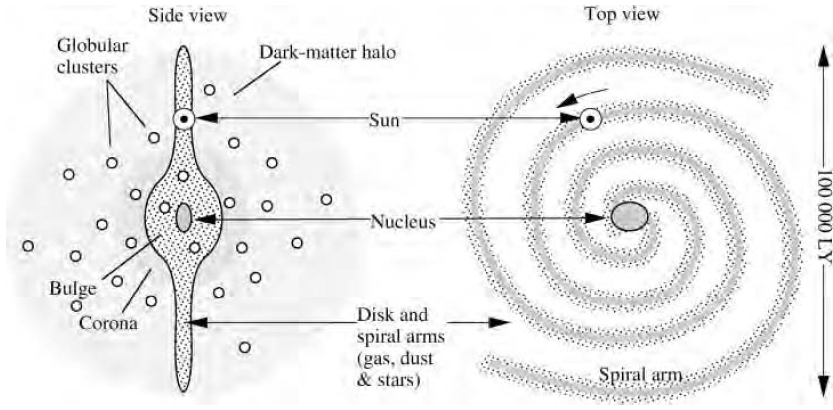
\includegraphics[width=0.49\textwidth]{./Immagini/Capitolo1/Via_Lattea_distr.png}
	\caption*{Distribuzione della massa nella Via Lattea}
	\vspace{-15pt}
\end{wrapfigure}

Parlando della nostra galassia, la Via Lattea, noi ci troviamo a circa $8.3\,kpc$ dal centro ed ha raggio di circa $30\,kpc$, è essenzialmente un disco molto piatto, per vederne il raggio e lo spessore è sufficiente plottare le luminosità acquisite nei survey in coordinate galattiche e studiare la distribuzione di massa in scala esponenziale con il raggio $r$ e lo spessore $h$, trovando la maggior concentrazione della massa entro i valori di $r_d=3.5\pm0.5\,kpc$ e $h_d\simeq160\,pc$.
\begin{equation*}
	\rho(r,z) = e^{ -\frac{r}{r_d}} e^{-\frac{|z|}{h_d}}
\end{equation*}
Vi sono poi ammassi globulari, ossia grappoli di stelle, distribuiti in modo approssimativamente sferico in un alone di materia oscura, quest'ultima fa da collante a questa distribuzione della materia nella galassia ed è facilmente rivelabile facendo una misura dinamica della massa, ossia misurando la velocità circolare di stelle a diversi raggi. La traiettoria terrestre nel piano galattico è in prima approssimazione circolare, con velocità lineare di $220\,km/s$ e periodo di rivoluzione attorno al centro galattico di $250$ milioni di anni, ma per avere queste velocità alla distanza $r_\odot=8\,kpc$ a cui noi ci troviamo, è necessario avere una massa dinamica di:
\begin{equation*}
	M(r<r_\odot) \simeq \frac{r_\odot v_\odot^2}{G} \simeq 10^{11}M_\odot
\end{equation*}
Mentre quella che è la massa stellare e delle polveri misurata è solo la metà di questo valore, si tiene conto infatti che la massa media delle stelle nella galassia è $<M>=0.5M_\odot$ e che le $10^{11}$ stelle che compongono la nostra galassia costituiscono il $90\%$ della massa misurabile, che è per tutto il disco galattico $M_{disk}=10^{10}M_\odot$.

\begin{wrapfigure}{r}{0.5\textwidth}
	%immagine presa dal Bradt - Astronomy Methods
	\vspace{-10pt}
	\centering
	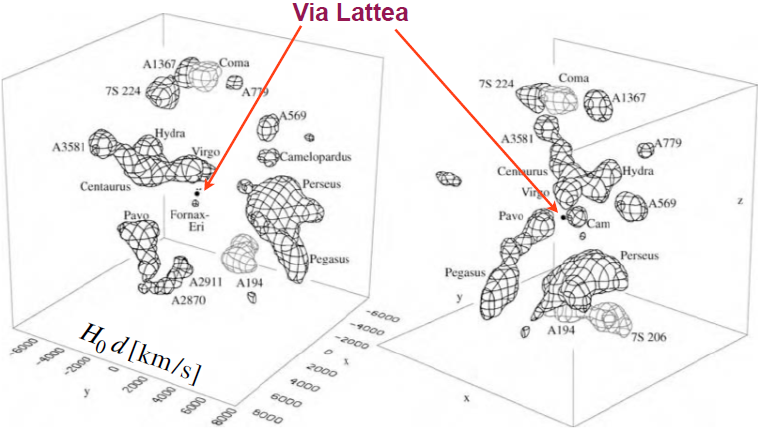
\includegraphics[width=0.49\textwidth]{./Immagini/Capitolo1/Gruppo_locale.PNG}
	\caption*{Distribuzione della massa nella Via Lattea}
	\vspace{-10pt}
\end{wrapfigure}

Per funzionamento "gerarchico" della gravità, anche le galassie si raccolgono in gruppi ed ammassi esattamente come le stelle, costruendo strutture, la nostra facendo parte del \textit{Gruppo Locale}, costituito da una sessantina di galassie gravitazionalmente legate tra loro. La famosa galassia Andromeda M31, una delle poche con dimensioni simili alla nostra e situata a circa $700\,kpc$ da noi, è all'estremo opposto del nostro gruppo, mentre circa la metà delle galassie del nostro gruppo sono a forma irregolare, altre sono sferoidali e solo tre hanno simmetria a spirale come la nostra. Allontanandoci di svariati $Mpc$, si va incontro ad altri gruppi ed agglomerati di galassie, superati la distanza di circa $100\,Mpc$, l'universo comincia ad essere abbastanza isotropo e ad avere un aspetto omogeneo, nel senso che questa tendenza al clustering (raggrupamento, granulosità) di stelle e poi galassie inizia a venire meno. Questa proprietà è fondamentale per comprendere l'universo tramite gli occhiali della relatività generale, teoria fondata sull'omogeneità dell'universo e grazie alla quale riusciamo a porre una descrizione analitica alle nostre osservazioni. 

\subsubsection*{Redshit e legge di Hubble}
Per parlare della scala dell'universo, dobbiamo introdurre la legge di Hubble, tornando indietro di cento anni nella storia. All'epoca, le altre galassie venivano catalogate a centinaia sotto il termine di nebule (o nebulose), chiedendosi se fossero parte della nostra galassia o fossero sistemi esterni. La svolta venne dalle osservazioni di Hubble ed i suoi collaboratori, tramite un telescopio di $2\,m$ di diametro e svolgendo studi di spettroscopia, analizzando una ventina di queste nebulose (galassie), di cui si aveva già una stimma della distanza da misurazioni indipendenti, e anallizando i loro effetti di \textbf{redshift}. Si ricorda che il redshift è interpretato tramite l'effetto Doppler, per cui:
\begin{equation*}
	z=\frac{\lambda_{obs}-\lambda_{em}}{\lambda_{em}}
\end{equation*}
Nel caso non relatistico $v \ll c$, il rapporto tra la differenza di lunghezza d'onda e la lunghezza d'onda originaria è data dal rapporto tra la velocità radiale di allontanamento della sorgente rispetto l'osservatore e la velocità della luce:
\begin{equation*}
	1+z = \frac{\lambda_{obs}}{\lambda_{em}} \overset{v \ll c}{=} 1+\frac{v}{c}
\end{equation*}
Quello che notò Hubble fu la correlazione lineare tra la velocità di recessione di queste galassie e la distanza a cui esse si trovano, dove la relazione osservativa si basa sulla costante di proporzione detta \textbf{costante di Hubble $H_0$}:
\begin{equation}
	\label{eq:Hubble}
	v_r=cz=H_0d
\end{equation}
Dove la costante viene misurata in $km/s/Mpc$ e la legge viene detta \textbf{legge di Hubble} (1930), risultato previsto teoricamente da Laimatre, tramite la risoluzione delle equazioni della relatività generale, e prova incisiva dell'espansione dell'universo, non più concepibile in modo statico come era diffusamente creduto all'epoca, anche dallo stesso Einstein. La legge deve subire chiaramente correzioni nelle applicazioni specifiche, per incontrare le influenze gravitazionali che le altre galassie del gruppo apportano a quella presa in considerazione, basti pensare alla citata Andromeda M31, la quale si avvicina alla nostra gallassia invece di recedere con velocità $v_r$. Nasce da questa legge, in una prima ipotesi abbozzata da Laimatre, il fatto che tornando a ritroso nel tempo, l'Universo si debba necessariamente contrarre, fino ad arrivare ad un punto in un tempo finito in cui la densità è inifinita, ossia la teoria del \textit{Big Bang}. Queste tempo è calcolato come l'inverso di $H_0$, chiaramente solo una stima, ma da l'idea dell'importanza di questa costante, in grado di dare sia la scala di espansione (e dimensionale) che la scala temporale dell'Universo, e la cui misura ha ricoperto una parte fondamentale nella fisica recente. Si accenna il fatto, per ragioni cosmologiche che non tratteremo, che da questa costante deriva anche la geometria dell'Universo. Queste prime deduzioni dalla legge di Hubble possono essere riassunte come:
\begin{align}
	\label{eq:Hubble-eta-uni}
	T_U   & \sim H_0^{-1} = \frac{1}{70km/s/Mpc} \simeq 4.3\e{17}s \simeq 14Gyr \\
	\label{eq:Hubble-grand-uni}
	L_H   & = cH_0^{-1} \simeq \frac{3\e{5}km/s}{70km/s/Mpc} \simeq 4200Mpc \simeq 10^{26}m \\
	\label{eq:Hubble-dens-uni}
	\rho_\varepsilon   & = \frac{3H_0^3}{8\pi G} \simeq 2\e{-29}g/cm^2
\end{align}
Chiaramente, queste scale di età e dimensioni dell'universo vanno interpretate più approfonditamente e corrette tramite la relatività generale.

Dalla legge di Hubble possiamo dedurre l'età delle sorgenti osservate in base al loro redshift, tecnica chiamata del \textit{Lookback time}. Osservando un corpo a distanza $d$, deriva che stiamo osservando fotoni, che viaggiando a velocità $c$, hanno impiegato un tempo:
\begin{equation*}
	t=\frac{d}{c}=\frac{z}{H_0}
\end{equation*}
Dove abbiamo sfruttato la \ref{eq:Hubble} per la seconda uguaglianza, ma sfruttando la \ref{eq:Hubble-eta-uni}, vediamo che il redshift fa da fattore di scala nello stimare l'età dei corpi osservati:
\begin{equation*}
	t=zT_U
\end{equation*}
Questa misurazione necessita comunque di correzioni relativistiche e cosmologiche per una stima più precisa, come già si era anticipato precedentemente. Noi oggi siamo arrivati ad una misurazione di oggetti con redshift dieci, ossia nati cinquecento di milioni di anni dopo il Big Bang, dove già a redshift sei vediamo sorgenti nate dopo un miliardo di anni, mentre a redshift pari a uno quelle con età pari alla metà di quella dell'universo. Il limite superiore, come si vede dal grafico, è di redshift venti, a cui si teorizza corrispondere la nascita delle prime stelle a duecento milioni di anni dal Big Bang. Le prime strutture più complesse, come i raggruppamenti stellari e successivamente le galassie, si formarono già verso redshift tre, mentre arrivando a uno l'universo era già molto simile a quello che è tutt'ora.

\chapter{Telescopi}

\section{Strutture dei telescopi e grandezze ottiche}

Per ora ci limiteremo a trattare i telescopi nella banda dell'ottico, anche se il discorso rimane molto simile anche per altre bande, essendo comunque basati sulla collezione di fotoni ad una certa lunghezza d'onda tramite riflessione su una superficie curva (processo di riflessione che risulta impossibile già con i raggi X). Le caratteristiche principali di un telescopio sono: sensibilità della misura (o flusso limite), potere risolutivo (ossia risoluzione angolare), campo di vista (o fov), larghezza di banda (determinata essenzialmente dallo strumento stesso), risoluzione spettrale.

\begin{wrapfigure}{l}{0.5\textwidth}
	%Immagine presa da slide
	\vspace{-10pt}
	\centering
	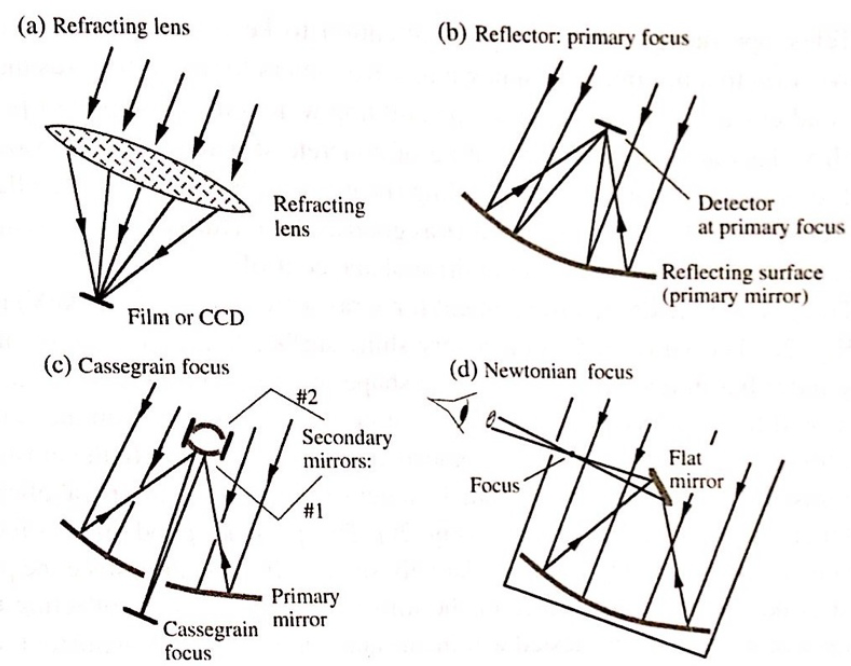
\includegraphics[width=0.49\textwidth]{./Immagini/Capitolo2/Telescopi_classici.png}
	\caption*{Telescopi classici nell'ottico}
	\vspace{-10pt}
\end{wrapfigure}

Dal punto di vista storico, sin dai tempi di Galileo i primi telescopi funzionavano a rifrazione, è necessario aspettare Newton per vedere i primi telescopi a riflessione, inizialmente basati su specchi sferici poi cambiati in parabolici per ridurre le aberrazioni generate dai primi. Di quest'ultima tipologia di telescopi, il più semplice e immediato è quello in cui il focus primario è messo immediatamente sopra lo specchio principale. Un altro modello che venne adottato frequentemente è quello di \textbf{Cassegrain}, in cui il fascio è ridirezione da uno specchio secondario, posto nello stesso punto in cui si trova il focus nel modello precedente, con riflessione del fascio in un buco dello specchio primario, un altro modello è quello a focus laterale e così via. Il motivo per cui si sono superati i telescopi rifrattori, è perchè necessariamente il telescopio dovrebbe essere lungo almeno quanto la lunghezza focale della lente, creando una strumentazione particolarmente ingombrante e scomoda. Un altro fattore non trascurabile è quello per cui questo tipo di lenti portano a un'aberrazione non trascurabile, inoltre questo tipo di telescopio deve essere necessariamente chiuso, contenendo la lente, ma il fascio focalizzato deve quindi attraversare una zona chiusa che per gradienti termici può creare moti convettivi che vanno a intaccare la bontà dell'osservazione, evitabili con una struttura aperta possibile solo con telescopi riflettivi. Si ricorda che per proprietà delle lenti, la \textbf{aberrazione cromatica} è il fenomeno per cui una lente ha indici di rifrazione diversi per lunghezze d'onda diverse, ciò genera un gradiente di colore, il che significa che a lunghezze focali sufficientemente grandi si ottengono punti di focus diversi a seconda della lunghezza d'onda osservata, anche nella stessa banda. Il problema è risolvibile aggiungendo sistemi di lenti correttrici il cui compito è proprio di rimuovere questo effetto di aberrazione, tecnica adoperabile ma che comporta costi aggiuntivi non indifferenti, anche per il fatto che a lenti sempre più grandi corrispondono costi e sistemi di correzione più grandi, possedendo questo un campo di vista maggiore ma anche effettivi di aberrazione maggiori.

\begin{wrapfigure}{r}{0.5\textwidth}
	\vspace{-10pt}
	\centering
	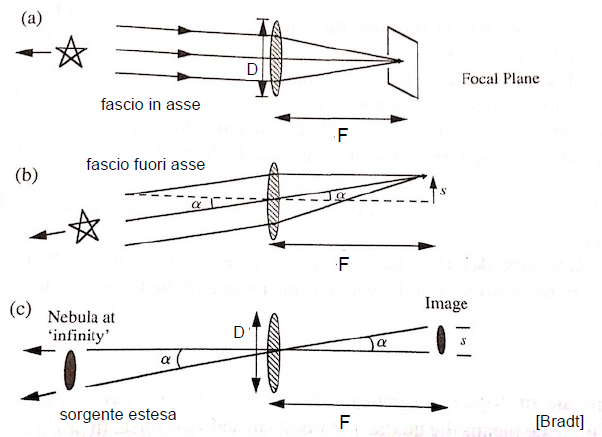
\includegraphics[width=0.49\textwidth]{Immagini/Capitolo2/Richiami_ottica_piano_focale.PNG}
	\vspace{-5pt}
	\caption*{Esempi di fasci e piano focale da sorgenti puntiformi ed estese}
	\vspace{-10pt}
\end{wrapfigure}

Facendo qualche richiamo di ottica, una lente focalizza un fascio incidente in asse con essa su un piano focale a distanza pari la lunghezza focale $F$, un fascio fuori asse di un angolo $\alpha$ verrà focalizzato a una distanza $F$ dalla lente e a una distanza $s$ dall'asse, dove:
\begin{equation*}
	s = F\tan\alpha \overset{\alpha\to0}{\simeq} F\cdot\alpha
\end{equation*}
In cui si può approsimare la tangente con l'angolo stesso per piccoli angoli. Ciò si applica alle sorgenti estese facendo combaciare il suo estremo superiore con l'asse focale e prendendo in riferimento per l'angolo $\alpha$ l'estremo inferiore, misurando in millimetri  (o in pixel tramite CCD) la distanza $s$, si trova la scala sul piano focale:
\begin{equation*}
	\frac{\Delta\alpha}{\Delta s} = \frac{1}{F}
\end{equation*}
Espressa in arcosecondi su millimetro (o su pixel), detto in inglese \textit{plate scale}(si ricordi che $\alpha$ è espresso in radianti e va convertito in arcosecondi). Si può definire una focale equivalente nota la distanza focale $F$ facendo semplicamente il rapporto tra un radiante (espresso in arcosecondi) e questa lunghezza. Un rapporto molto importante è il \textit{rapporto focale} $f$ definito come:
\begin{equation*}
	f=\frac{F}{D}
\end{equation*}
Dove $D$ è il diametro della lente focalizzante. Questa grandezza è particolarmente importante in quanto il suo inverso $\/f$ determina la "velocità" della lente, di fatti una lente con lunghezza focale maggiore focalizzerà l'immagine su un numero di pixel $s$ maggiore a parità di angolo $\alpha$ di deviazione dall'asse, essendo le due in proporzionalità diretta. Nei tempi di esposizione, un'immagine e quindi un flusso distribuito su più pixel necessiterà di un'esposizione maggiore per avere un buono rapporto segnale-rumore, questo significa che una lente con rapporto $1/f$ piccolo, avrà lunghezza focale $F$ grande, e perciò sarà più lenta. Nel caso reale entra in gioco anche l'area collettrice, ossia le dimensioni del telescopio, le quali determinano la quantità di flusso a cui è esposto il rivelatore su cui mette a fuoco al lente. Questo significa che se un'immagine ha dimensioni lineari $s$, avrà area proporzionale a $s^2$, per cui l'energia del fotone focalizzato per ogni pixel sarà proporzionale al rapporto tra le dimensioni dell'apertura che permette il passaggio del fotone e quelle dell'immagine su cui questo fotone va a "distribuirsi":
\begin{equation*}
	E_{ph} \propto \frac{D^2}{s^2} \propto \frac{D^2}{F^2} = f^{-2}
\end{equation*}
Questo esprime che una lente con rapporto focale $f$ di piccole dimensioni, avrà grande apertura e lunghezza focale corta, per cui avrà bisogno di tempi di esposizione minori ma al tempo stesso avrà una capacità risolutiva e di distinzione degli oggetti minore, godendo però di un campo visivo (fov) maggiore, essendo l'apertura $D$ maggiore. Riassumendo, per ricordare meglio, un rapporto $f^{-1}$ piccolo corrisponde ad una piccola velocità di acquisizione, mentre un valore grande di questo parametro corrisponde a una grande velocità di acquisizione.

\begin{wrapfigure}{r}{0.5\textwidth}
	%Immagine presa da slide
	\vspace{-10pt}
	\centering
	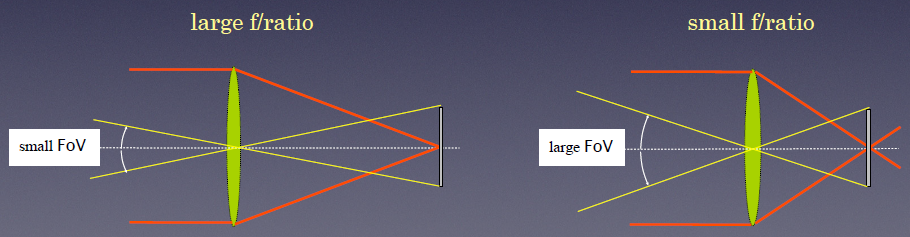
\includegraphics[width=0.49\textwidth]{Immagini/Capitolo2/fov.png}
	\caption*{Esempi di fov correlati a $f$}
	\vspace{-10pt}
\end{wrapfigure}

Un'altra proprietà collegato al rapporto focale è il \textit{campo di vista}, o \textit{fov} (field of view), proporzionale anch'esso a $f$. Di fatti, oltre che la scala sul piano focale e il tempo di esposizione, il rapporto determina per ragioni geometriche facilmente intuibili il campo di vista in modo inversamente proporzionale, per cui a un grande valore di $f$ corrisponde un piccolo campo visivo, mentre per un valore minore un campo maggiore. Correlandolo con la velocità, una lente veloce (f piccolo) avrà un campo di vista più grande, viceversa un più lenta (f grande) avrà campo di vista minore. Questo implica che le prime sono più adatte ad un'osservazione meno dettagliata ma di porzioni di cielo maggiori, mentre le seconde sono particolarmente apprezzate nella risoluzione di porzioni di cielo ed oggetti specifici. Parlando di telescopi esistenti e futuri, il telescopio POSS è stata la principale fonte di informazione per i surveys in tutto il cielo stellato fino agli anni '60, possiede $f/2.5$ e lenti correttrici, ossia è una telescopio molto veloce e ad ampio fov. Un altro esempio più recente, di inizio millennio, è il telescopio SDSS con $f/5$, per cui più lenta e precisa, che ha permesso un grande numero di scoperte nell'interstellare fino alle scale cosmologico, coprendo cinque bande nell'ottico. Attualmente in uso c'è il telescopio VISTA in Cile per il vicino infrarosso con $f/3.3$, che errà presto sostituito dal LSST entro il 2021, con $f/1.25$ (estremamente veloce e ad ampio fov). Un parametro che stima l'efficienza nella velocità di acquisizione sempre maggiore di queste macchine è il "grasp" (o "etendue" dal francese), che è l'efficienza della macchina a osservare una certa zona di cielo entro un certo flusso limite ed è definita come:
\begin{equation*}
	Grasp = D^2 \cdot FoV \, (m^2 \cdot deg^2)
\end{equation*}
Maggiore è questo parametro maggiore sarà la velocità con cui è capace di effetture osservazioni il telescopio in oggetto. Chiaramente è direttamente proporzionale al fov in quanto si tratta di un parametro osservativo, mentre tiene conto del flusso limite tramite il termine $D^2$.

\subsubsection*{Aberrazioni ottiche}

Sia la lente che le camere poste davanti il punto focale che costituiscono il telescopio sono fortemente influenzate degli effetti di aberrazione accennati precedentemente e che ora accenneremo più in dettaglio.

\begin{wrapfigure}{l}{0.5\textwidth}
	\vspace{-10pt}
	\centering
	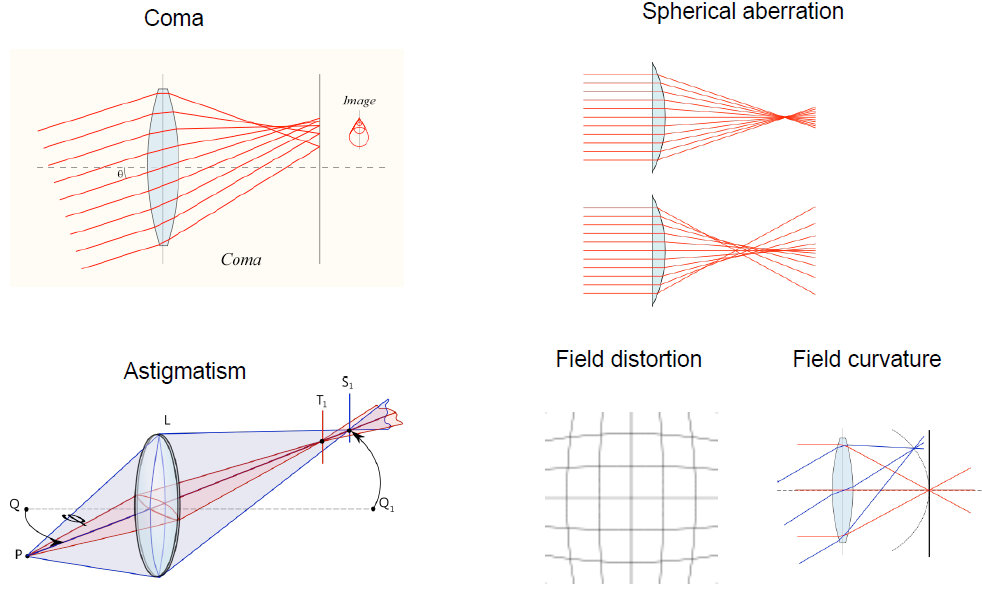
\includegraphics[width=0.49\textwidth]{Immagini/Capitolo2/Aberrazioni.png}
	\caption*{Tipologie di aberrazioni ottiche}
	\vspace{-10pt}
\end{wrapfigure}

Le principali tipologie di aberrazioni ottiche, riassunte in figura, sono il \textit{coma}, l'aberrazione sferica, l'astigmatismo, la distorsione di campo e la curvatura di campo. La prima riguarda i raggi del fascio incidente più fuori asse rispetto a quelli centrali, per cui succede che per conformazione della lente convergente i corrispettivi raggi rifratti non vadano a convergere nello stesso punto, creando una piccola coda. L'\textit{aberrazione sferica} riguarda la forma della lente, per cui i raggi più distanti dall'asse ottico vengono rifratti ad angoli diversi andando a convergere in punti diversi rispetto quello focale (dove comunque confluiscono tutti i raggi che in incidenza erano più vicini l'asse). L'\textit{astigmatismo} consiste nella perdita di simmetria assiale, per cui raggi incidenti ad angoli diversi convergono a distanze focali diverse. Altri tipi di aberrazione, come quella della \textit{curvatura di campo}, procudono effetti distortivi per cui il piano focale diventa curvo, problema tipico dei telescopi a fov molto grandi e risolvibile con le moderne tecnologie creando appositi CCD curvi. Questo effetto si ritrova similmente nella \textit{distorsione di campo}, effetto che fa perdere la scala di misure del piano focale sull'intero campo di vista, come è facilmente dall'immagine, e per cui si ottengono pixel equivalenti che non hanno le stesse dimensioni costanti in tutto il campo di vista. Questi effetti possono essere limitati in principio creando strumentazioni apposite, ad esempio usando specchi parabolici anzichè sferici nei telescopi riflessivi. In generale, si parla di fov corretto per i indicare il fov di un telescopio una volta aggiunte le strumentazioni e applicate tutte quelle correzioni che puntano a ridurre gli effetti di queste aberrazioni.

% ragiona se rifare i paragrafi o mettere la prossima parte (struttura di cassegrain e telescopi riflessivi) nella parte prima delle aberrazioni o boh

\subsection{Telescopi riflessivi}

Il più comune dei telescopi riflessivi è il Cassegrain, citato prima, dove il fascio viene riflesso da uno specchio principale su un secondario convesso, il quale riflette a sua volta i raggi sul piano focale attraversando un buco nello specchio primario. Combinando gli effetti riflessivi dei due specchi, si può ricavare la correlazione tra le distanze focali tramite la seguente:
\begin{equation*}
	\frac{1}{F_p-d}=\frac{1}{d}+\frac{1}{F_s}
\end{equation*}
Dove $F_p$ è la distanza focale dello specchio primario, $F_s$ del secondario e $d$ la distanza a cui è interposto il secondo specchio convesso rispetto al punto focale del primo.

\begin{wrapfigure}{r}{0.4\textwidth}
	\vspace{-10pt}
	\centering
	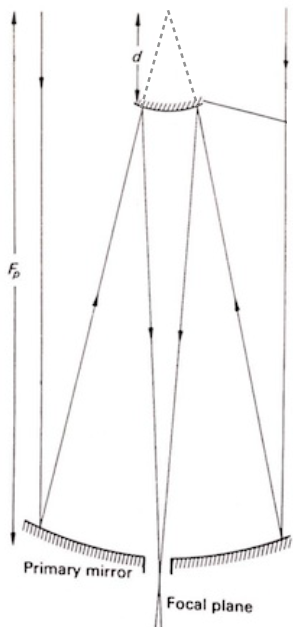
\includegraphics[width=0.35\textwidth]{Immagini/Capitolo2/Cassegrain.PNG}
	\caption*{Schema del modello Cassegrain}
	\vspace{-20pt}
\end{wrapfigure}

Come accennato al paragrafo precedente, gli specchi sono parabolici per favorire la convergenza di tutti i raggi nello stesso punto focale, anche quelli maggiormente fuori asse. Lo svantaggio di questa struttura sta nell'ingombro che lo specchio secondario comporta, riducendo notevolmente il campo visivo. Un design di questa tipologia di telescopi particolarmente diffusa è quella di \textbf{Ritchey-Chrétien}, basato su strutture iperboliche per entrambi gli specchi che annullano l'aberrazione sferica e il coma, riducendo al tempo stesso l'astigmatismo e la curvatura di campo, mantenendo un fov corretto abbastanza ampio. Un altro vantaggio di questa struttura è la sua compattezza, riducendo i costi di costruzione e di sviluppo della meccanica atta a mantenerne la stabilità e a muoverlo per coprire varie parti di cielo. Il prezzo principale di questo modello è uno specchio secondario maggiore, che arriva a coprire anche il $20\%$ del campo di vista rispetto ad altri.

\subsubsection*{Risoluzione angolare e funzione di risposta}

Per definire il concetto di risoluzione angolare di un telescopio, è necessario fare ulteriori richiami di ottica. Un fenomeno importante ai fini della definizione di questo parametro è la \textit{diffrazione di Fraunhofer}, storicamente adoperata per la comprensione della natura della luce, se questa fosse corpuscolare o ondulatoria, il cui scopo è quello di indagare gli effetti che ha una fenditura su un fronte d'onda piano. Innanzitutto, per fronte d'onda si intendono dei punti nello spazio ugualmente distanziati in cui l'onda si trova nella stessa fase, ad esempio i fronti di picco sono quelli in cui l'onda si ritrova periodicamente ad avere dei picchi in punti ben definiti dello spazio. Una volta che questi fronti d'onda colpiscono una fenditura, quello che si osserva è la generazione di frange di interferenza costruttive e distruttive, interpretato da Fraunhofer come effetto di interferenza tra le onde che vengono generate in ogni punto della fenditura, che diventa quindi sorgente.

\begin{wrapfigure}{l}{0.5\textwidth}
	\vspace{-10pt}
	\centering
	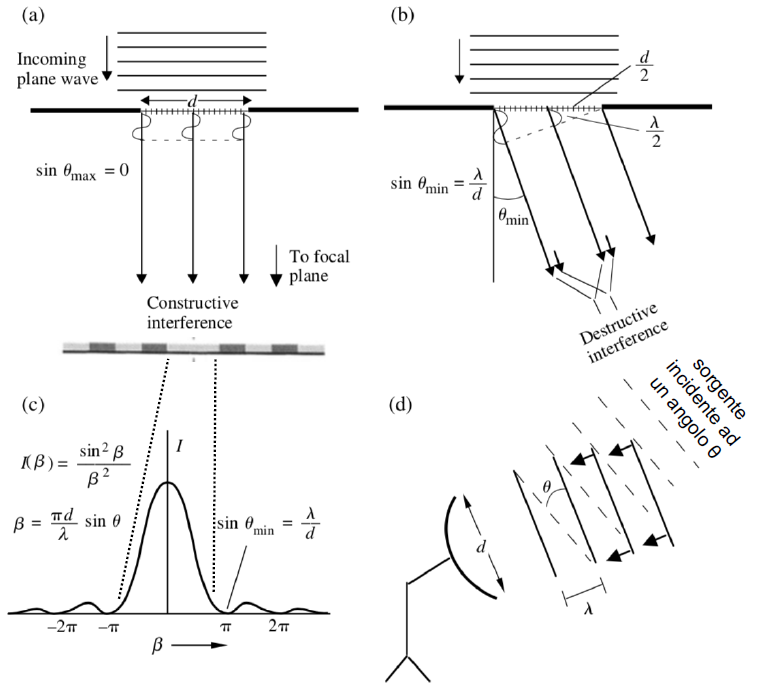
\includegraphics[width=0.49\textwidth]{Immagini/Capitolo2/Fraunhofer.PNG}
	\caption*{Diffrazione di Fraunhofer}
	\vspace{-10pt}
\end{wrapfigure}

Nel caso i fronti incidano perpendicolarmente la fenditura, le onde generate in asse saranno speculari a quelle incidenti, per cui avremmo frange ad interferenza costruttiva nelle proiezioni sul piano focale, come mostrato in figura. Nel caso la sorgente non sia in asse con la fenditura bisogna calcolare lo sfasamento di ogni fronte generato nei diversi punti di essa. Per fare questa misura bisogna considerare la differenza di cammino $\Delta s$ all'inizio della propagazione, come mostrato nella (b), tra le due onde prese in considerazione e prendendo in riferimento la congiungente ortogonale la direzione di propagazione rispetto a cui si vuole trovare l'interferenza risultante. Dalla trigonometria sappiamo che la differenza di cammino generante lo sfasamento è:
\begin{equation*}
	\Delta s = \frac{a}{2}\sin\theta
\end{equation*}
Dove abbiamo considerato le due onde come distanti metà fenditura l'una dall'altra, come nella (b), e dove $a$ è la grandezza della fenditura, $\theta$ l'angolo sotteso tra la normale alla fenditura e l'asse scelto in direzione del piano focale. Nel caso di interferenza distruttiva, le onde dovranno essere perfettamente in antifase, ossia avere una differenza di fase di $\pi$, ma essendo che le onde sono descritte da funzioni periodiche con periodo $t=2\pi$, per avere tale sfasamento dovremmo misurare una differenza di cammino pari a $\lambda/2$. Il risultato è un picco centrale luminoso seguito da zone di buio e poi nuovamente a interferenza costruttiva di dimensioni e intensità via via minori, quello che si trova per l'andamento dell'intensità di luce è:
\begin{equation*}
	I(\beta) = \frac{\sin^2(\beta)}{\beta^2} \qquad \text{dove} \,
	\beta = \frac{\pi d}{\lambda}\sin\theta
\end{equation*}
Dove chiaramente per $\theta$ nullo si ha il primo e maggiore picco, mentre per $\beta=\pi$, ossia $\sin\theta=\lambda/d$, si ha il primo minimo. Essendo i telescopi, così come anche le antenne radio e altri rivelatori, costituiti da fenditure circolari che fanno ostruzione e originano diffrazione con il segnale entrante, questo fenomeno è cruciale nella definizione di risoluzione angolare. Le sorgenti talmente vicine da avere separazione angolare vicina al rapporto tra la lunghezza d'onda del fascio incidente e il diametro del telescopio, produrranno uno sfasamento da una parte all'altra dell'entrata del telescopio (causante ostruzione). Nel caso questa differenza di percorso $\Delta s$ diventi più piccola della lunghezza d'onda stessa, non saremo più in grado di distinguere i due segnali, essendo i loro picchi di diffrazione troppo sovrapposti per essere distinguibili.

\begin{wrapfigure}{l}{0.3\textwidth}
	\vspace{-5pt}
	\centering
	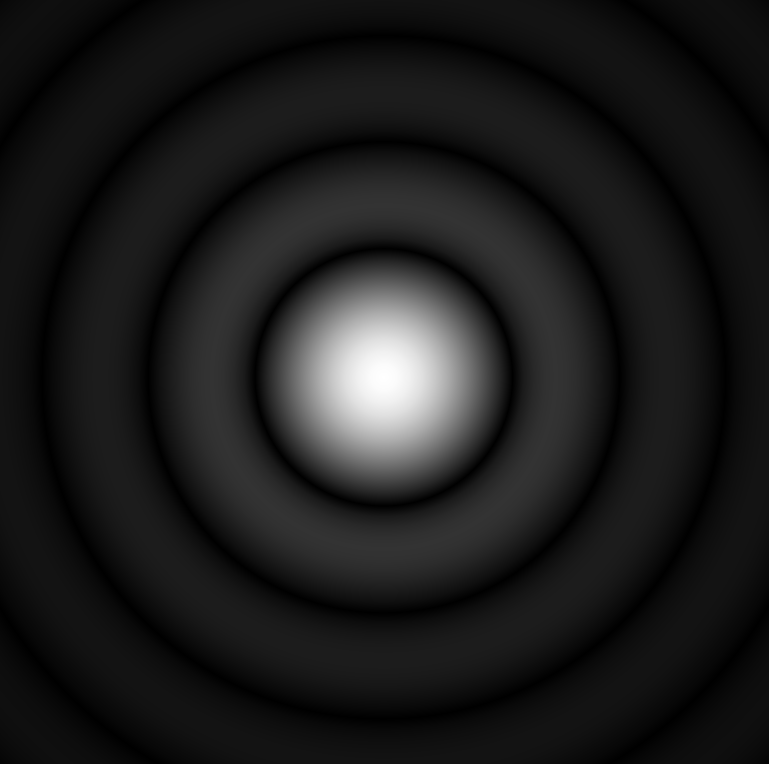
\includegraphics[width=0.29\textwidth]{Immagini/Capitolo2/Disco_Airy.PNG}
	\caption*{Disco di Airy}
	\vspace{-12pt}
\end{wrapfigure}

Risolvendo gli integrali di Wessel relativi alla fenditura circolare (caso proprio dei telescopi) viene fuori un rapporto numerico che relaziona l'angolo a cui si forma il primo minimo di diffrazione con il rapporto $\lambda/d$ tramite il fattore di forma:
\begin{equation*}
	\alpha_{min}=1.22\frac{\lambda}{d}
\end{equation*}
Dove chiaramente il pattern di diffrazione ha simmetria circolare, anzichè la disposizione a bande analizzata prima, creando il cosiddetto \textit{Disco di Airy}. Da ciò, si introduce il concetto di \textbf{risoluzione angolare} tramite il criterio di Rayleigh, secondo cui un telescopio con apertura $d$ è in grado di risolvere due sorgenti di lunghezza d'onda $\lambda$ se esse si trovano non più vicine tra loro della distanza a cui si trova il primo minimo di diffrazione, in formula se la loro separazione angolare $\Delta\alpha$ è al massimo:
\begin{equation*}
	\Delta\alpha = \alpha_{min} = 1.22\frac{\lambda}{d}
\end{equation*}
Considerato anche il rumore di fondo presente nelle osservazioni, di norma è difficile visualizzare il secondo disco di massimo a meno che la fonte non sia particolarmente luminosa. Questo secondo picco può essere particolarmente fastidioso nel caso la rivelazione punti all'osservazione di un pianeta legato a una stella, che se posto abbastanza vicino la stella rischia di essere oscurato, in tal caso si aggiunge anche il fatto che mediamente il contrasto tra un pianeta e la propria stella è di circa un fattore dieci. 

\begin{wrapfigure}{l}{0.4\textwidth}
	\vspace{-10pt}
	\centering
	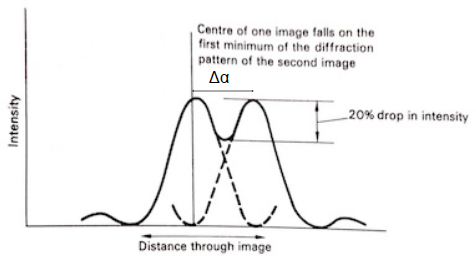
\includegraphics[width=0.39\textwidth]{Immagini/Capitolo2/Risoluzione_angolare.PNG}
	\caption*{RIsoluzione angolare in termini del pattern di diffrazione}
	\vspace{-5pt}
\end{wrapfigure}

Come parametro della risoluzione angolare ma anche del fit gaussiano del profilo di luminosità di una stella si usa la $FWHM$ (full width half maximum) del primo massimo di interferenza. Il discorso è più complesso per i telescopi da terra, particolarmente limitati dalla turbolenza atmosferica, mentre per quelli posti in orbita il discorso di esaurisce proprio in questi termini, dove si ricorda che la deviazione standard $\sigma$ di una gaussiana è correlata alla $FWHM$ secondo la relazione $\sigma=2.355\, FWHM$. Per capire la sua importanza basta vedere il plot del pattern di diffrazione (intensità percepita sul piano focale in funzione della distanza), in cui viene rappresentato il caso limite in cui il picco della seconda sorgente cade esattamente dove si trova il primo minimo di diffrazione della prima sorgente, in questo caso le sorgenti si sovrappongono proprio nel punto di FWHM citato prima.

\begin{exrc}[Sonda Cassini e Saturno]
	La sonda Cassini, in orbita attorno Saturno da diversi anni, è finita due volte nelle condizioni geometriche tali da avere un'eclissi totale del Sole da parte del pianeta, in tal modo si sono potute fare osservazioni della lontana Terra, avendo la principale sorgente di luce del nostro sistema oscurata. Su questa sonda sono posti due telescopi, uno angolo ampio molto veloce (WAC - wide angle camera), e uno a focale maggiore e campo di vista minore (NAC - narrow angle camera), che hanno rispettivamente $F=20\, cm$ e $f/3.5$, $F=2\, cm$ e $f/10.5$, mentre i CCD danno pixel di $12\, \mu m$. Ora la distanza di Saturno in quell'istante era $d=1.44\e{12}m$, mentre la distanza tra la Terra e la Luna media è $T-L=3.84\e{8}m$. Si chiede di trovare:
	\begin{enumerate}
		\item Qual è la scala in arcsec/pixel in WAC e NAC?
		\item Quanti arcsec (e pixel) separano la Terra dalla Luna nelle immagini WAC e NAC?
		\item Risoluzione angolare di WAC e NAC
		\item La Terra e’ risolta nelle immagini ?
	\end{enumerate}
\end{exrc}
\begin{sol}
	Suddividiamo la soluzione nei rispettivi punti posti nell'esercizio:
	\begin{enumerate}
		\item Scala in arcsec/pixel in WAC e NAC:
		\begin{itemize}
			\item Scala WAC: $\frac{206265}{200mm}=1031"/mm=12.4"/pixel$
			\item Scala NAC: $\frac{206265}{2000mm}=103.1"/mm=1.2"/pixel$
		\end{itemize}
		\item Separazione Terra-Luna nei due telescopi:
		\begin{itemize}
			\item WAC:
			\item Scala NAC:
		\end{itemize}
		\item Risoluzioni angolari di WAC e NAC:
		\begin{itemize}
			\item WAC:
			\item Scala NAC:
		\end{itemize}
		\item La Terra?
	\end{enumerate}
\end{sol}


\end{document}